\documentclass[10pt, letterpaper, titlepage]{article}
% \documentclass[10pt, letterpaper, titlepage]{report}

% % Packages
\input{../../packages.tex}
\input{../../commands.tex}
\input{../../setup.tex}

% \usepackage{hyperref} % Doesn't like math in section titles
% \newcommand{\smath}[2]{\texorpdfstring{#1}{#2}} % Use this to not break hyperref

% \setcounter{secnumdepth}{-1} % Sets sectioning level for numbering 
% % -1 part     1 section     3 subsubsection  5 subparagraph
% %  0 chapter  2 subsection  4 paragraph

% % Debug
% % For \hbox too wide errors.
% \overfullrule=.01cm

% Header
\geometry{margin = 1in}
\pagestyle{fancy}
\headheight = 23.01503pt
\lhead{}
\rhead{Yifeng Pan
     \\Draft. Not for Submission. UCID: 30063828}

% Title page
\title{Math 355 Assignment 3}
\author{Instructor: Dr Ryan Hamilton
    \\Name: Yifeng Pan
    \\UCID: 30063828}
\date{Fall 2019}

\begin{document}
    \maketitle

    \section{Suppose $S \subseteq \R$.}
    \subsection{Show that if $S \neq \R$ and $S \neq \emptyset$, then $\bd(S) \neq \emptyset$.}
        We prove the contrapositive: 
        If $\bd(S) = \emptyset$, then $S = \R$ or $S = \emptyset$.
        Suppose $\bd(S) = \emptyset$.
        If $S = \emptyset$, we are done.
        Let $S \neq \emptyset$. We prove $S = \R$.
        Since $\bd(S) = \emptyset$, $S = \interior(S)$.
        Since $S \neq \emptyset$, let $x_1 \in S$.
        Since $x_1$ is an interior point of $S$,
        $\lis \e_1$ such that $(x_1 - \e_1, x_1 + \e_1) \subseteq S$.
        Let $x_2 = x_1 + \e_1$.
        If $x_2 \not\in S$, then $x_2$ would be a boundary point of $S$,
        which would be a contradiction.
        Therefore $x_2 \in S$.
        We repeat to construct the sequence $\set{x_n}$, and $\set{\e_n}$,
        such that $x_{n+1} > x_n$, 
        and if $x_n < y < x_{n+1}$, then $y \in N_{\e_n}(x_n) \subseteq S$.
        Therefore, $\lall n, [x_1, x_n) \subseteq S$.
        As $n \to \infty$, 
        if $\set{x_n}$ is convergent to $L$, then $L$ is a boundary point of $S$,
        which is a contradiction.
        Therefore $\set{x_n}$ is divergent to infinity, as it's increasing.
        Therefore $[x_1, \infty) \subseteq S$.
        Simularly, we construct the sequence in the negative direction to prove
        $(-\infty, x_1] \subseteq S$.
        Therefore $S = \R$.

    \subsection{Show that $\bd(S) = \overline{S} \intersection \overline{\R \setminus S}$.}
        We know $\bd(S) = \bd(\R \setminus S)$, 
        As they have the same definition.

        % \begin{lemma}
        %     $\bd(S) \subseteq  \overline{S} \intersection \overline{\R \setminus S}$
        % \end{lemma}
            % Proof:
            Suppose $x \in \bd(S)$.
            Since $\bd{S} \subseteq \overline S$,
            $x\in \overline S$.
            Since $x \in \bd(S) = \bd(\R \setminus S)$,
            $x \in \overline{\R \setminus S}$.
            Therefore $x \in \overline{S} \intersection \overline{\R \setminus S}$.
            % \qed

        % \begin{lemma}
        %     $\overline{S} \intersection \overline{\R \setminus S} \subseteq \bd(S)$
        % \end{lemma}
            % Proof:
            Suppose 
            $x \in \overline{S} \intersection \overline{\R \setminus S}
                = (S \union \bd(S)) \intersection ((\R \setminus S \union \bd(\R \setminus S))$.
            Therefore $x \not\in S \lif x \in \bd(S)$
            and $x \in S \lif x \not\in \R \setminus S \lif x \in \bd(\R \setminus S) = \bd(S)$.
            Therefore $x \in \bd(S)$ is both cases.
            % \qed

        Therefore
        $\bd(S) = \overline{S} \intersection \overline{\R \setminus S}$.
    % \newpage
    \section[Problem 2]{}
    \subsection[(i)]{Using the division algorithm, find the greatest common divisor of $x^4 + x + 1$
        and $x^3 + 2$ in $\Q[x]$ and express it as a linear combination of these polynomials. 
        Explain your computation.}
        % \footnote{Reference: \url{https://en.wikipedia.org/wiki/Polynomial_long_division}}
        \begin{center}
            \begin{tabular}{|c|c|c|c|c|}
                \hline
                $\bm{i}$& $\bm{r}$          & $\bm{s}$  & $\bm{t}$  & $\bm{q} = r_{i-1} / r_i$ \\
                \hline
                $0$ & $x^4 + x + 1$                         & $1$  & $0$  & \----  \\
                \hline
                $1$ & $x^3 + 2$                             & $0$  & $1$  & $x$    \\
                \hline
                $2$ & $(x^4 + x + 1) - x(x^3 + 2) = -x+1$   & $1$  & $-x$  & $-x^2$ \\
                \hline
                $3$ & $(x^3 + 2) -(- x^2)(-x+1) = x^2 + 2$  & $x^2$& $1-x^3$  & $0$    \\
                \hline
                $4$ & $(-x+1) -0(x^2 + 2) = -x+1$           & $1$  & $-x$  & $-x$   \\
                \hline
                $5$ & $(x^2+2) - (-x)(-x+1) = x+2$          & $x^2+x$  & $1-x^3-x^2$  & $-1$   \\
                \hline
                $6$ & $(-x+1) - (-1)(x+2) = 3$              & $1+x^2+x$  & $1-x^3-x^2-x$   & $(x+2)/3$  \\
                \hline
                $7$ & $(x+2) - ((x+2)/3)(3) = 0$            & $s_5 - s_6q_6$  & $t_5 - t_6q_6$  & \----  \\
                \hline
            \end{tabular}
        \end{center}
        
        \footnote{Reference: \url{https://en.wikipedia.org/wiki/Polynomial_greatest_common_divisor\#B\%C3\%A9zout's_identity_and_extended_GCD_algorithm}}
        where
        $s_5 - s_6q_6 = (x^2+x) - \frac{x+2}{3}(1+x^2+x) = \frac{- x^3 - 2}{3}$, 
        \footnote{Calculator: \url{https://www.symbolab.com/}.}
        \\
        and 
        $t_5 - t_6q_6 = (1-x^3-x^2) - \frac{x+2}{3}(1-x^3-x^2 - x) = \frac{x^4+x+1}{3}$.

        $r_6 = 3 = r_0s_6 + r_1t_6 = (x^4+x+1)(1+x^2+x) + (x^3+2)(1-x^3-x^2-x)$.

        $\gcd(x^4+x+1, x^3 + 2) = 1$ (Multiply the above by $1/3$).

    \subsection[(ii)]{Let $P,Q \in \Z[x]$. Prove that $P$ and $Q$ are relatively prime in $\Q[x]$
        if and only if the ideal $(P,Q)$ of $\Z[x]$ generated by $P$ and $Q$ contains a non-zero integer
        (i.e. $\Z \intersection (P,Q) \neq \set{0})$. Here $(P,Q)$ is the smallest ideal of $\Z[x]$
        containing $P$ and $Q$, $(P,Q) = \set{\alpha P + \beta Q | \alpha, \beta \in \Z[x]}$
    }
        Suppose $P$ and $Q$ are relatively prime in $\Q[x]$.

        By definition of relatively prime, $\lis p(x), q(x) \in \Q[x]$ (henceforth refered to as $p,q$)
        such that $pP + qQ = 1$.

        But $p = a/b$ for some $a \in \Z[x], b \in \N$
        \footnote{Let $b$ be the lowest common multiple of the denominators of the coefficients of
            $p$ in their irreducible fraction forms.}
        ,
        and $q = c/d$ for some $c \in \Z[x], d \in \N$.

        So $pP + qQ = adP + cbQ = bd$, where $ad, cb \in \Z[x], bd \in \N$.
        Therefore $bd \in (P,Q)$.

        Now, Suppose $(P,Q)$ contains a non-zero integer $n \in \Z \setminus\set{0}$.

        So $\lis a,b \in \Z[x]$ such that $aP + bQ = n$.

        So for $a/n, b/n \in \Q[x]$, $a/n P + b/n Q = 1$.

        Therefore $P$ and $Q$ are relatively prime in $\Q[x]$.
        \qed

    \subsection[(iii)]{For which primes $p$ and which integers $n\geq 1$ is the polynomial 
        $x^n - p$ irreducible in $\Q[x]$? Justify your answer.}

        Let $p$ be a prime. Let $n \geq 1$.

        By the Eisenstein Criterion: 
        \footnote{Artin's Algebra, Proposition 12.4.6, Eisenstein Criterion.}
        \\
        Since $p$ divides $-p$, $p^2$ does not divide $-p$, and $p$ does not divide $1$,
        $(1)x^n + (-p) = x^n - p$ in irreducible in $\Q[x]$.
        \qed
    \section{R has a built-in dataset called {\color{red} trees} that contains observations for 
    $n = 31$ black cherry
    trees. The first column, “Girth,” contains the girth of the trees (in inches); the second
    column, “Height,” contains the height of the trees (in feet); the third column, “Volume,”
    contains the volume of timber (in cubic feet).}
    \begin{multicols}{2}
        \subsection{State the least-squares estimate of the model predicting diameter from height.}
            (Note: Diameter is mislabeled as girth in the dataset.)\\
            $d$ and $h$ are in inches: $d \approx 0.02131h-6.188$

        \subsection{Predict the diameters of trees of the following heights: 
            $60$ feet, $73$ feet, and $85$ feet.}
            In inches.\\
            Height of 60 feet: \\
            $d \approx 0.02131226 (60 * 12)-6.18839451$
            $\approx 9.156$\\
            Height of 73 feet: \\
            $d \approx 0.02131226 (73 * 12)-6.18839451$
            $\approx 12.48$\\
            Height of 85 feet: \\
            $d \approx 0.02131226 (85 * 12)-6.18839451$
            $\approx 15.55$

        \subsection{Interpret the meaning of the slope in the context of the data.}
            For every 1 inch increase the height, 
            there will be a 0.02131 inch increase in diameter.

        \subsection{Suppose you wanted to conduct a hypothesis test for a positive linear relationship
            between height and diameter. State the appropriate hypotheses and test statistic.}
            $H_0: \beta_1 \leq 0, H_a: \beta_1 > 0$\\
            $t = \frac{\beta_1 - \beta_{1_0}}{SE_{\beta_1}}
            \approx \frac{0.02131226 - 0}{ 0.006513191} \approx 3.272$

        \subsection{State the probability expression of the p-value as well as the p-value itself. What
            conclusion would we reach with respect to our hypotheses in part d. using $\alpha = 0.05$?}
            $\pv = P(T_{df} > 3.272\hdots) = 1 - pt(t, df) 
            \approx 0.1379\% < 5\% = \alpha$\\
            Therefore there is a linear dependency of height on diameter.

        \subsection{If you wanted to report a $95\%$ interval for the diameter of a single tree that was $80$
            feet tall, would you report a confidence interval or prediction interval? Why?}
            Prediction interval, as it predicts the dependent variable 
            from a given independent variable\\
            Prediction interval: (13.08276, 15.45999 ) in inches.

        \subsection{What proportion of $\sigma^2$ in diameter is explained by its linear relationship with
            height?}
            $r^2 \approx 0.2697$

        \subsection{Examine the residual plot. What condition/assumption does the residual plot check for?
            Does it appear to be met in this case?}
            %See figure \ref{fig:3h} on page \pageref{fig:3h}.
            It checks for consistancy in variance. 
            In this case, yes, the points are in a random pattern.
            \begin{center}
                % Created by tikzDevice version 0.12.3 on 2019-08-18 21:40:24
% !TEX encoding = UTF-8 Unicode
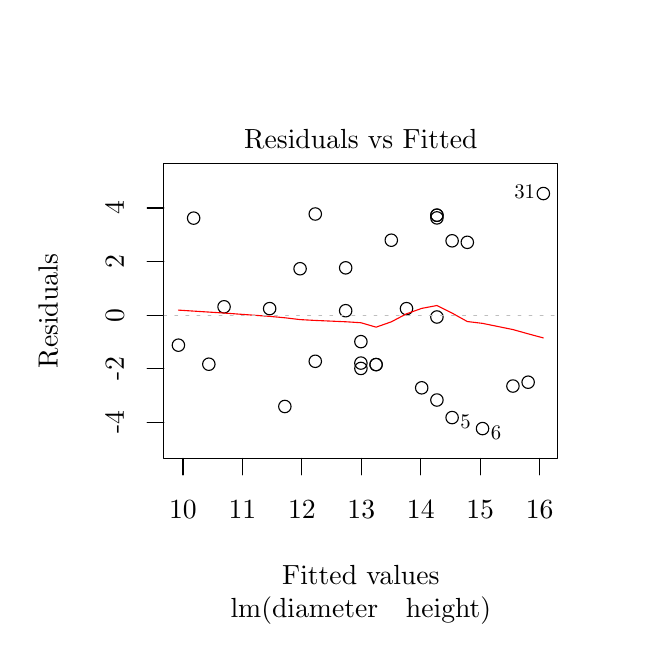
\begin{tikzpicture}[x=1pt,y=1pt]
\definecolor{fillColor}{RGB}{255,255,255}
\path[use as bounding box,fill=fillColor,fill opacity=0.00] (0,0) rectangle (216.81,216.81);
\begin{scope}
\path[clip] (  0.00,  0.00) rectangle (216.81,216.81);
\definecolor{drawColor}{RGB}{0,0,0}

\path[draw=drawColor,line width= 0.4pt,line join=round,line cap=round] ( 56.11, 61.20) -- (185.01, 61.20);

\path[draw=drawColor,line width= 0.4pt,line join=round,line cap=round] ( 56.11, 61.20) -- ( 56.11, 55.20);

\path[draw=drawColor,line width= 0.4pt,line join=round,line cap=round] ( 77.60, 61.20) -- ( 77.60, 55.20);

\path[draw=drawColor,line width= 0.4pt,line join=round,line cap=round] ( 99.08, 61.20) -- ( 99.08, 55.20);

\path[draw=drawColor,line width= 0.4pt,line join=round,line cap=round] (120.56, 61.20) -- (120.56, 55.20);

\path[draw=drawColor,line width= 0.4pt,line join=round,line cap=round] (142.05, 61.20) -- (142.05, 55.20);

\path[draw=drawColor,line width= 0.4pt,line join=round,line cap=round] (163.53, 61.20) -- (163.53, 55.20);

\path[draw=drawColor,line width= 0.4pt,line join=round,line cap=round] (185.01, 61.20) -- (185.01, 55.20);

\node[text=drawColor,anchor=base,inner sep=0pt, outer sep=0pt, scale=  1.00] at ( 56.11, 39.60) {10};

\node[text=drawColor,anchor=base,inner sep=0pt, outer sep=0pt, scale=  1.00] at ( 77.60, 39.60) {11};

\node[text=drawColor,anchor=base,inner sep=0pt, outer sep=0pt, scale=  1.00] at ( 99.08, 39.60) {12};

\node[text=drawColor,anchor=base,inner sep=0pt, outer sep=0pt, scale=  1.00] at (120.56, 39.60) {13};

\node[text=drawColor,anchor=base,inner sep=0pt, outer sep=0pt, scale=  1.00] at (142.05, 39.60) {14};

\node[text=drawColor,anchor=base,inner sep=0pt, outer sep=0pt, scale=  1.00] at (163.53, 39.60) {15};

\node[text=drawColor,anchor=base,inner sep=0pt, outer sep=0pt, scale=  1.00] at (185.01, 39.60) {16};

\path[draw=drawColor,line width= 0.4pt,line join=round,line cap=round] ( 49.20, 74.25) -- ( 49.20,151.66);

\path[draw=drawColor,line width= 0.4pt,line join=round,line cap=round] ( 49.20, 74.25) -- ( 43.20, 74.25);

\path[draw=drawColor,line width= 0.4pt,line join=round,line cap=round] ( 49.20, 93.60) -- ( 43.20, 93.60);

\path[draw=drawColor,line width= 0.4pt,line join=round,line cap=round] ( 49.20,112.95) -- ( 43.20,112.95);

\path[draw=drawColor,line width= 0.4pt,line join=round,line cap=round] ( 49.20,132.31) -- ( 43.20,132.31);

\path[draw=drawColor,line width= 0.4pt,line join=round,line cap=round] ( 49.20,151.66) -- ( 43.20,151.66);

\node[text=drawColor,rotate= 90.00,anchor=base,inner sep=0pt, outer sep=0pt, scale=  1.00] at ( 34.80, 74.25) {-4};

\node[text=drawColor,rotate= 90.00,anchor=base,inner sep=0pt, outer sep=0pt, scale=  1.00] at ( 34.80, 93.60) {-2};

\node[text=drawColor,rotate= 90.00,anchor=base,inner sep=0pt, outer sep=0pt, scale=  1.00] at ( 34.80,112.95) {0};

\node[text=drawColor,rotate= 90.00,anchor=base,inner sep=0pt, outer sep=0pt, scale=  1.00] at ( 34.80,132.31) {2};

\node[text=drawColor,rotate= 90.00,anchor=base,inner sep=0pt, outer sep=0pt, scale=  1.00] at ( 34.80,151.66) {4};

\path[draw=drawColor,line width= 0.4pt,line join=round,line cap=round] ( 49.20, 61.20) --
	(191.61, 61.20) --
	(191.61,167.61) --
	( 49.20,167.61) --
	( 49.20, 61.20);
\end{scope}
\begin{scope}
\path[clip] (  0.00,  0.00) rectangle (216.81,216.81);
\definecolor{drawColor}{RGB}{0,0,0}

\node[text=drawColor,anchor=base,inner sep=0pt, outer sep=0pt, scale=  1.00] at (120.41, 15.60) {Fitted values};

\node[text=drawColor,rotate= 90.00,anchor=base,inner sep=0pt, outer sep=0pt, scale=  1.00] at ( 10.80,114.41) {Residuals};
\end{scope}
\begin{scope}
\path[clip] ( 49.20, 61.20) rectangle (191.61,167.61);
\definecolor{drawColor}{RGB}{0,0,0}

\path[draw=drawColor,line width= 0.4pt,line join=round,line cap=round] ( 92.93, 79.92) circle (  2.25);

\path[draw=drawColor,line width= 0.4pt,line join=round,line cap=round] ( 65.46, 95.20) circle (  2.25);

\path[draw=drawColor,line width= 0.4pt,line join=round,line cap=round] ( 54.47,102.08) circle (  2.25);

\path[draw=drawColor,line width= 0.4pt,line join=round,line cap=round] (103.92, 96.26) circle (  2.25);

\path[draw=drawColor,line width= 0.4pt,line join=round,line cap=round] (153.37, 75.92) circle (  2.25);

\path[draw=drawColor,line width= 0.4pt,line join=round,line cap=round] (164.36, 71.94) circle (  2.25);

\path[draw=drawColor,line width= 0.4pt,line join=round,line cap=round] ( 70.96,115.95) circle (  2.25);

\path[draw=drawColor,line width= 0.4pt,line join=round,line cap=round] (120.41, 93.67) circle (  2.25);

\path[draw=drawColor,line width= 0.4pt,line join=round,line cap=round] (147.88, 82.26) circle (  2.25);

\path[draw=drawColor,line width= 0.4pt,line join=round,line cap=round] (120.41, 95.61) circle (  2.25);

\path[draw=drawColor,line width= 0.4pt,line join=round,line cap=round] (142.38, 86.67) circle (  2.25);

\path[draw=drawColor,line width= 0.4pt,line join=round,line cap=round] (125.90, 95.07) circle (  2.25);

\path[draw=drawColor,line width= 0.4pt,line join=round,line cap=round] (125.90, 95.07) circle (  2.25);

\path[draw=drawColor,line width= 0.4pt,line join=round,line cap=round] ( 87.44,115.29) circle (  2.25);

\path[draw=drawColor,line width= 0.4pt,line join=round,line cap=round] (120.41,103.35) circle (  2.25);

\path[draw=drawColor,line width= 0.4pt,line join=round,line cap=round] (114.91,114.53) circle (  2.25);

\path[draw=drawColor,line width= 0.4pt,line join=round,line cap=round] (175.35, 87.31) circle (  2.25);

\path[draw=drawColor,line width= 0.4pt,line join=round,line cap=round] (180.84, 88.70) circle (  2.25);

\path[draw=drawColor,line width= 0.4pt,line join=round,line cap=round] ( 98.43,129.70) circle (  2.25);

\path[draw=drawColor,line width= 0.4pt,line join=round,line cap=round] ( 59.97,147.99) circle (  2.25);

\path[draw=drawColor,line width= 0.4pt,line join=round,line cap=round] (136.89,115.28) circle (  2.25);

\path[draw=drawColor,line width= 0.4pt,line join=round,line cap=round] (147.88,112.26) circle (  2.25);

\path[draw=drawColor,line width= 0.4pt,line join=round,line cap=round] (114.91,130.02) circle (  2.25);

\path[draw=drawColor,line width= 0.4pt,line join=round,line cap=round] (103.92,149.48) circle (  2.25);

\path[draw=drawColor,line width= 0.4pt,line join=round,line cap=round] (131.39,140.01) circle (  2.25);

\path[draw=drawColor,line width= 0.4pt,line join=round,line cap=round] (153.37,139.79) circle (  2.25);

\path[draw=drawColor,line width= 0.4pt,line join=round,line cap=round] (158.86,139.25) circle (  2.25);

\path[draw=drawColor,line width= 0.4pt,line join=round,line cap=round] (147.88,148.07) circle (  2.25);

\path[draw=drawColor,line width= 0.4pt,line join=round,line cap=round] (147.88,149.04) circle (  2.25);

\path[draw=drawColor,line width= 0.4pt,line join=round,line cap=round] (147.88,149.04) circle (  2.25);

\path[draw=drawColor,line width= 0.4pt,line join=round,line cap=round] (186.34,156.87) circle (  2.25);
\definecolor{drawColor}{RGB}{255,0,0}

\path[draw=drawColor,line width= 0.4pt,line join=round,line cap=round] ( 54.47,114.75) --
	( 59.97,114.39) --
	( 65.46,114.04) --
	( 70.96,113.69) --
	( 87.44,112.49) --
	( 92.93,111.98) --
	( 98.43,111.32) --
	(103.92,111.02) --
	(103.92,111.02) --
	(114.91,110.54) --
	(114.91,110.54) --
	(120.41,110.19) --
	(120.41,110.19) --
	(120.41,110.19) --
	(125.90,108.59) --
	(125.90,108.59) --
	(131.39,110.51) --
	(136.89,113.41) --
	(142.38,115.37) --
	(147.88,116.41) --
	(147.88,116.41) --
	(147.88,116.41) --
	(147.88,116.41) --
	(147.88,116.41) --
	(153.37,113.67) --
	(153.37,113.67) --
	(158.86,110.62) --
	(164.36,109.96) --
	(175.35,107.72) --
	(180.84,106.18) --
	(186.34,104.70);
\end{scope}
\begin{scope}
\path[clip] (  0.00,  0.00) rectangle (216.81,216.81);
\definecolor{drawColor}{RGB}{0,0,0}

\node[text=drawColor,anchor=base,inner sep=0pt, outer sep=0pt, scale=  1.00] at (120.41,  3.60) {lm(diameter ~ height)};
\end{scope}
\begin{scope}
\path[clip] (  0.00,  0.00) rectangle (216.81,216.81);
\definecolor{drawColor}{RGB}{0,0,0}

\node[text=drawColor,anchor=base,inner sep=0pt, outer sep=0pt, scale=  1.00] at (120.41,173.01) {Residuals vs Fitted};
\end{scope}
\begin{scope}
\path[clip] (  0.00,  0.00) rectangle (216.81,216.81);
\definecolor{drawColor}{RGB}{0,0,0}

\node[text=drawColor,anchor=base east,inner sep=0pt, outer sep=0pt, scale=  0.75] at (183.34,155.15) {31};

\node[text=drawColor,anchor=base west,inner sep=0pt, outer sep=0pt, scale=  0.75] at (167.36, 67.92) {6};

\node[text=drawColor,anchor=base west,inner sep=0pt, outer sep=0pt, scale=  0.75] at (156.37, 71.90) {5};
\end{scope}
\begin{scope}
\path[clip] ( 49.20, 61.20) rectangle (191.61,167.61);
\definecolor{drawColor}{RGB}{190,190,190}

\path[draw=drawColor,line width= 0.4pt,dash pattern=on 1pt off 3pt ,line join=round,line cap=round] ( 49.20,112.95) -- (191.61,112.95);
\end{scope}
\end{tikzpicture}

            \end{center}
    \end{multicols}
    \section[Problem 4]{}
    \subsection[(i)]{List the even permutations in the symmetric group of degree $4$,
        i.e. the elements of the alternating group $A_4$. How many of them are of order $3$?}
        
        \begin{align*}
            p(\vectorvalue{1,2,3,4})
            \in \{
                &\vectorvalue{1,2,3,4},
                \vectorvalue{1,3,4,2},
                \vectorvalue{1,4,2,3},\\
                &\vectorvalue{2,1,4,3},
                \vectorvalue{2,3,1,4},
                \vectorvalue{2,4,3,1},\\
                &\vectorvalue{3,1,2,4},
                \vectorvalue{3,2,4,1},
                \vectorvalue{3,4,1,2},\\
                &\vectorvalue{4,1,3,2},
                \vectorvalue{4,2,1,3},
                \vectorvalue{4,3,2,1}\}
        \end{align*}
        \footnote{Source: \url{https://groupprops.subwiki.org/wiki/Element_structure_of_alternating_group:A4}}
        There are $8$ of order $3$.

    \subsection[(ii)]{Let $G$ be a group. Show that a subgroup $H$ of $G$ of index $2$ is necessarily normal.}
        \footnote{Source: \url{https://proofwiki.org/wiki/Subgroup_of_Index_2_is_Normal}}
        Let $H$ be a subgroup of $G$, and $\abs{G:H} = 2$.

        Since the index is $2$, partition $G$ into $H, H'$, 
        so $H \union H' = G$, and $H \intersection H' = \emptyset$.

        Let $g \in G$.

        If $g \in H$, then $gH = Hg$, and we're done.

        Suppose $g \in H'$.
        Then $gH = H'$, otherwise $H = H'$.
        Similarly $Hg = H'$.
        Therefore $gH = H' = Hg$.

        Therefore $H$ is a normal subgroup of $G$.
        \qed


    \subsection[(iii)]{Let $K$ be a subgroup of $A_4$ of order $6$. Show that for all $a \in A_4$,
        the cosets $K, aK,$ and $a^2K$ cannot all be distinct, and deduce that $K$ must necessarily
        contain all elements of order $3$ of $A_4$. Conclude that $A_4$ does not have a subgroup of 
        order $6$, even though $6$ divides the order of $A_4$.}
        
        \footnote{Source: \url{https://math.stackexchange.com/questions/582658/a-4-has-no-subgroup-of-order-6}}
        Let $K$ be a subgroup of $A_4$.
        Let $\abs{K} = 6$.

        % Since $\abs{G:K} = 2$, $K$ is normal.
        

        If $K, aK, a^2K$ are all distinct, then $\abs{G:H} \geq 3$, but $\abs{G:H} = 2$.
        Therefore $K, aK, a^2K$ are not all distinct.
        \qed

        Since there are $8$ elements of order $3$ in $A_4$,
        and $K$ only contains $6$ elements,
        choose $a \in A_4, a \not\in K$, and the order of $a = 3$.

        Suppose $K = aK$.
        Since $1 \in K, a = a1,$ and $a \in K$.
        Contradiction.

        Suppose $K = a^2K$.
        Similarly $a^2 \in K$, but $K$ is a group, so ${(a^2)}^{-1} = a \in K$.
        Contradiction.

        Suppose $aK = a^2K$.
        Similarly $a(a) = a^2 (1) $, so $a \in K$.
        Contradiction.

        Therefore $K$ must necessarily contain all $a\in A_4$ of order $3$.\\
        Therefore the subgroup $K$ of $A_4$ such that $\abs{K}= 6$ does not exist.
        \qed
    \section[Problem 5]{Recall our notation for the dihedral group $D_n, n \geq 1$.
    We have $x,y\in D_n$ such that the orders $o(x) = n, o(y)=2, yx = x^{-1}y$ and $D_n = <x,y>$.}
    \subsection[(i)]{Write down the element $x^2yx^{-1}y^{-1}x^3y^3$ of $D_n$
        in the form $x^iy^i$, for integers $i,j \geq 0$.}

        We have $x^n = 1, y^2 = 1, yx = x^{-1}y$.
        Now, 
        \begin{align*}
            yx &= x^{-1}y \\
            y &= x^{-1}y x^{-1} \\
            xy &= y x^{-1} \\
            % 
            \to & x^2yx^{-1}y^{-1}x^3y^3 \\
            = & x^2yx^{-1}y^{-1}x^3y \\
            = & x (y x^{-1}) x^{-1}y^{-1}x^2 (y x^{-1}) \\
            = & x y x^{-2}y^{-1}x^2 y x^{-1} \\
            = & y x^{-3}y^{-1} y x^{-3} \\
            = & y x^{-3} x^{-3} \\
            = & y x^{-6} \\
            = & x^6 y \\
            \to & i = 6, j = 1
        \end{align*}


    \subsection[(ii)]{Let $G$ be a group. Show that for all $a\in G$, if the subset $\set{1,a}$
        is a normal subgroup of $G$ then $a$ is in the center of $G$.
        Prove that $N = \set{1, x^5}$ is a normal subgroup of $D_{10}$.}
        
        Suppose $a\in G$ such that $\set{1,a}$ is a normal subgroup of $G$.
        % So $\lall g \in G, gag^{-1} \in \set{1,a}$.

        Let $x \in G$.
        Since $\set{1,a}$ is a normal subgroup of $G, xax^{-1} \in \set{1,a}$.
        If $xax^{-1} = a$, then $xa = ax$, we're done.
        If $xax^{-1} = 1$, then $a = 1$, so $xa = ax$.
        \qed

        % We need to prove $N = \set{1,x^5}$ is a normal subgroup of $D_{10}$.

        We have $x,y \in D_{10}, x^{10} = 1, y^2 = 1, yx = x^{-1}y$.

        Let $h \in N = \set{1,x^5}$. $h = 1$ is the trivial case, so assume $h = x^5$.

        Now, $x x^5 x^{-1} = x^5 \in N$, and $y x^5 y^{-1} = x^{-5} y y^{-1} = x^{-5} = x^5 \in N$.
        And any combination of $x$ and $y$ would yield the same result.
        Therefore $N$ is a normal subgroup of $D_{10}$.
        \qed
        
        

    \subsection[(iii)]{Compute the left cosets of $N$ in $D_{10}$ and show that the quotient group
        $\frac{D_{10}}{N}$ is isomorphic to $D_5$.}

        \(
            \set{
                \set{1, x^5},
                \set{x, x^6},
                \set{x^2, x^7},
                \set{x^3, x^8},
                \set{x^4, x^9},
                \set{y, yx^5},
                \set{yx, yx^6},
                \set{yx^2, yx^7},
                \set{yx^3, yx^8},
                \set{yx^4, yx^9}
            }
        \).

        We find a bijective group homomorphism from $D_{10}/N$ to $D_5$.

        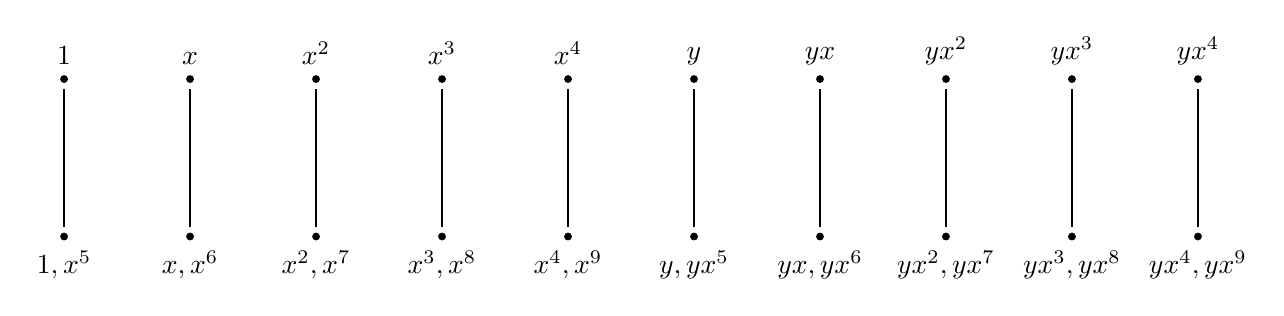
\begin{tikzpicture}[
            ele/.style={fill=black,circle,minimum width=.8pt,inner sep=1pt}
        ]
            \node[ele,label=above:$1$] (b1) at (0,2) {};
            \node[ele,label=above:$x$] (b2) at (1.6,2) {};    
            \node[ele,label=above:$x^2$] (b3) at (3.2,2) {};
            \node[ele,label=above:$x^3$] (b4) at (4.8,2) {};
            \node[ele,label=above:$x^4$] (b5) at (6.4,2) {};
            \node[ele,label=above:$y$] (b6) at (8,2) {};
            \node[ele,label=above:$yx$] (b7) at (9.6,2) {};    
            \node[ele,label=above:$yx^2$] (b8) at (11.2,2) {};
            \node[ele,label=above:$yx^3$] (b9) at (12.8,2) {};
            \node[ele,label=above:$yx^4$] (b10) at (14.4,2) {}; 

            \node[ele,label=below:$\set{1, x^5}$] (a1) at (0,0) {};
            \node[ele,label=below:$\set{x, x^6}$] (a2) at (1.6,0) {};    
            \node[ele,label=below:$\set{x^2, x^7}$] (a3) at (3.2,0) {};
            \node[ele,label=below:$\set{x^3, x^8}$] (a4) at (4.8,0) {};
            \node[ele,label=below:$\set{x^4, x^9}$] (a5) at (6.4,0) {};
            \node[ele,label=below:$\set{y, yx^5}$] (a6) at (8,0) {};
            \node[ele,label=below:$\set{yx, yx^6}$] (a7) at (9.6,0) {};    
            \node[ele,label=below:$\set{yx^2, yx^7}$] (a8) at (11.2,0) {};
            \node[ele,label=below:$\set{yx^3, yx^8}$] (a9) at (12.8,0) {};
            \node[ele,label=below:$\set{yx^4, yx^9}$] (a10) at (14.4,0) {}; 

            \draw[thick,shorten <=2pt,shorten >=2pt] (a1) -- (b1);
            \draw[thick,shorten <=2pt,shorten >=2pt] (a2) -- (b2);
            \draw[thick,shorten <=2pt,shorten >=2pt] (a3) -- (b3);
            \draw[thick,shorten <=2pt,shorten >=2pt] (a4) -- (b4);
            \draw[thick,shorten <=2pt,shorten >=2pt] (a5) -- (b5);
            \draw[thick,shorten <=2pt,shorten >=2pt] (a6) -- (b6);
            \draw[thick,shorten <=2pt,shorten >=2pt] (a7) -- (b7);
            \draw[thick,shorten <=2pt,shorten >=2pt] (a8) -- (b8);
            \draw[thick,shorten <=2pt,shorten >=2pt] (a9) -- (b9);
            \draw[thick,shorten <=2pt,shorten >=2pt] (a10) -- (b10);
        \end{tikzpicture}
        \qed
    \section[Problem 6]{
    Let $p$ be a prime number.
}  
    \subsection[(i)]{
        Show that there are $\frac{p(p+1)}{2}$ reducible monic quadratic polynomials over
        the finite field $\F_p = \Z/p\Z$.
    }
        Monic quadratic polynomials are of the form $x^2 + ax + b$, for some $c,d\in \F_p$.

        There are $p^2$ polynomials of this form in $\F_p$.

        Since quadratics are of degree $2$, the are either irreducible,
        or can be reduced into two polynomials with degree $1$.

        Therefore the reducible polynomials are of the form 
        $x^2 + ax + b = (x + c)(x + d) = x^2 + (c+d)x + cd$, for some $c,d \in \F_p$.

        % The number of distinct reducible polynomials are therefore the number of distinct
        % solutions to the equations $c+d = a, cd = b$, $a,b,c,d \in \F_p$.

        The number of distinct reducible polynomials are therefore the number of distinct
        images of $(x+c)(x+d)$ with $c,d \in \F_p$.

        We count:
        \begin{enumerate}
            \item Choose $c \in \F_p$. ($p$ choices)
            \item Choose $d \in \F_p, d \neq c$. ($p - 1$ choices)
            \item The choices for $(c,d)$ are commutative, so we counted everything twice. ($1/2$)
            \item Now we add the the number of ways to choose $c,d\in \F_p, c= d$. ($p$ choices).
        \end{enumerate}

        We have $\frac{p(p-1)}{2} + p = \frac{p^2 - p + 2p}{2} = \bm{\frac{p(p+1)}{2}}$.
        \qed





    \subsection[(ii)]{
        Construct a field of order $49$.
    }
        $F = \F_7 / (x^2 + 1)$.

        Since $x^2 + 1$ has degree $2$, if it is reducible, it can be reduced into
        two polynomials of degree $1$, which would imply it has integer roots.

        It's easy to check that $x^2 + 1 \neq 0, \lall x \in \set{0,1,2,3,4,5,6} = \F_7$.
        Therefore $x^2 + 1 $ is irreducible in $\F_7$.

        Since $x^2 + 1$ is irreducible in $\F_7$, $F$ is a field.
        \footnote{I proved this in Assignment 5, 
            I've provided a copy of the proof on the next page.}

        Since $x^2 + 1$ kills all the polynomials of above degree $2$ in $\F_7$,
        all the elements of $F$ are of the form $ax + b, a,b \in \F_7$.

        Therefore $\abs{F} = 7^2 = 49$.
        \qed

    \subsection[(iii)]{
        Is there a field $F$ of characteristic $p$ such that $F$ is an infinite set?
        Prove that $F$ does not exist or give an example.
    }
        We know $\Z/2\Z[x]$ is an integral domain.

        Define $F$ as a field of fractions over $\Z/2\Z[x]$.

        $F$ is a field by construction.

        We have to prove $F$ is infinite with a characteristic $2$.

        Let $[\frac{a}{b}]\in F$, for $a,b\in \Z/2\Z[x], b \neq 0$.

        $[\frac{a}{b}] + [\frac{a}{b}] = [\frac{2a}{b}] = [\frac{0}{b}]$, since $2a = 0 \in \Z/2\Z[x]$,
        where $[\frac{0}{b}]$ is the additive identity in $F$.

        Therefore $F$ has a characteristic of $2$.

        Now, we construct an infinite subset of $F$.
        Let $S = \set{[\frac{x}{1}],[\frac{x^2}{1}],[\frac{x^3}{1}],[\frac{x^4}{1}],\hdots} \subseteq F$.

        The elements of $S$ are all distinct equivalence classes, i.e. elements of $F$,
        since $x^a 1 \neq x^b 1, \lall a,b\in \N, a\neq b$.

        Since $S$ is denumerable,
        $F$ is not finite.
        \qed



\section*{Lemma used in (6.2)}
    \begin{lemma}
        $\F_p[x] / (f(x))$ is a field $\iff$ $f(x)$ is irreducible in $\F_p[x]$.
    \end{lemma}
        Proof:
        Suppose $f(x) \in \F_p[x]$ is irreducible (henceforth refered to as $f$).

        Let $[g] \in \F_p[x]/(f)$, where $g \in \F_p[x] \setminus \set{0}$.
        We find the inverse of $[g]$.

        Since $f$ is irreducible, $\gcd(f, g) = c$ for some constant $c \in \F_p$.
        Otherwise, $c$ would be a non-constant factor of $f$.

        By Bézout's Identity: \\
        $\lis a, b \in \F_p[x]$, such that 
        $af + bg = 1$.
        Now, 
        \begin{align*}
            [af + bg] &= [1] \\
            % [af] + [bg] &= [1] \\
            [a][f] + [b][g] &= [1] \\
            [a][0] + [b][g] &= [1] \\
            % af + bg + (f) &= 1 + (f) \\
            % bg + (f) &= 1 + (f) \\
            [b][g] &= [1]
        \end{align*}
        Therefore $[b]$ is the multiplicative inverse of $[g]$ in $\F_p[x] / (f)$,
        where $[1]$ is the multiplicative identity.

        Since $\F_p[x] / (f)$ is a quotient ring, and since every element has an inverse,
        $\F_p[x] / (f)$ is a field.

        Now for the logical inverse: Suppose $f$ is reducible.
        So $\lis$ non-constants $a,b \in F_p[x]$ such that $ab = f$.
        
        We have
        \(
            [ab] = [f] \to
            [a][b] = [0]
        \).

        Suppose $[a] = [0]$.
        So $\lis r \in \F_p[x]$, such that $rf = a$.
        Now, $ab = f \to rfb = f$,
        and since we know $\F_p[x]$ is an integral domain, $rb = 0$.
        But $r \neq 0$, $b \neq 0$ from construction
        ($r\neq 0$ because $a \neq 0$)
        ,so $\F_p[x]$ has non-zero zero divisors.
        Contradiction.

        Therefore $[a] \neq [0]$.
        Similarly, $[b] \neq [0]$.

        Since $[a] \neq [0]$ and $[b] \neq [0]$, $\F_p[x] / (f)$ has non-zero zero divisors,
        and therefore is not an integral domain, 
        and therefore not a field.
        \qed

    \section{Supoose $A$ and $B$ are both bounded subsets of $\R$. Find an property $\meta{X}$ so that
    the statement $\sup A = \inf B$ if and only if $\meta{X}$ is true.}
    
    Property $\meta{X}$: $\forall a \in A, \forall b \in B, a \leq b$ 
    AND $\forall \epsilon \in \R, \epsilon >0, \exists x \in A, y \in B$ such that $y - x < \epsilon$.

    If $\meta{X}$ then $\sup A = \inf B$. Proof: \\ 
    Suppose $\meta{X}$.
    Suppose $\sup A > \inf B$. 
    We know that $\forall a \in A, \forall b \in B, a \leq b$.
    Therefore $\inf B$ is an upper-bound of $A$.
    Contradiction. 
    Now suppose $\sup A < \inf B$.
    Now, set $\epsilon = \inf B - \sup A > 0$.
    Then $\forall a \in A, b\in B: b - a \geq \sup B - a \geq \sup B - \inf A = \epsilon$.
    Therefore $b - a \not < \epsilon$. 
    Contradiction.
    Therefore $\sup A = \inf B$.

    If $\sup A = \inf B$ then $\meta{X}$. Proof: \\ 
    Suppose $\sup A = \inf B$.
    This means that $\forall a \in A , b \in B, a \leq \sup A = \inf B \leq b$.
    Now, let $\epsilon \in \R, \epsilon > 0$.
    We know $\exists x \in A$ such that $x > \sup A - \epsilon/2$ (otherwise $\sup A - \epsilon/2$ would be a upper bound).
    We also know that $\exists y \in B$ such that $y < \inf B + \epsilon/2$ (otherwise $\inf B + \epsilon/2$ would be a lower bound).
    Now, 
    \begin{align*}
        \epsilon &= \epsilon + \inf B - \inf B \\ 
        &= (\inf B + \frac{\epsilon}{2}) - (\inf B - \frac{\epsilon}{2}) \\ 
        &= (\inf B + \frac{\epsilon}{2}) - (\sup A - \frac{\epsilon}{2}) \\ 
        &> y - (\sup A - \frac{\epsilon}{2}) \\ 
        &> y - x \\ 
    \end{align*}
    Therefore $\meta{X}$.

    Therefore $\sup A = \inf B$ IFF $\meta{X}$.
    \section{Suppose $f$ is continuous on $[a,b]$ where $a<b$
     and let $M = \sup_{a\leq x \leq b} (\abs{f(x)})$.}

     \subsection{If $M > 0$ and $p$ is any positive constant,
        show that for every $\e > 0$
        there are constants $c<d$ 
        so that $[c,d] \subseteq [a,b]$
        and
        \[
            \bm{
                (M-\e)^p (d-c) 
                \leq 
                \int_a^b \abs{f(x)}^p dx 
                \leq
                M^p(d-a)
            }
        \]
    }

    \subsection{Prove that
        \[
            \bm{
                \lim_{p\to \infty}\left(\int_a^b \abs{f(x)}^p dx \right )^{\frac{1}{p}} = M
            }
        \]
    }

\end{document}
